	\documentclass[10pt,oneside]{CBFT_book}
	% Algunos paquetes
	\usepackage{amssymb}
	\usepackage{amsmath}
	\usepackage{graphicx}
	\usepackage{libertine}
	\usepackage[bold-style=TeX]{unicode-math}
	\usepackage{lipsum}

	\usepackage{natbib}
	\setcitestyle{square}

	\usepackage{polyglossia}
	\setdefaultlanguage{spanish}


	\usepackage{CBFT.estilo} % Cargo la hoja de estilo

	% Tipografías
	% \setromanfont[Mapping=tex-text]{Linux Libertine O}
	% \setsansfont[Mapping=tex-text]{DejaVu Sans}
	% \setmonofont[Mapping=tex-text]{DejaVu Sans Mono}

	%===================================================================
	%	DOCUMENTO PROPIAMENTE DICHO
	%===================================================================

\begin{document}

% =================================================================================================
\chapter{Relatividad especial}
% =================================================================================================

% =================================================================================================
\section{Transformación de vectores}
% =================================================================================================

Digamos que un vector transforma 
\[
	X'_{i} = a_{ij} X_j
\]
de manera que se verifique que las leyes físicas sean invariantes frente a rotaciones propias.

Einstein postula que:
\begin{itemize}
 \item Todos los sistemas inerciales son equivalentes.
 \item La velocidad de la luz en un sistema inercial es constante. No depende del estado de
 movimiento del observador.
\end{itemize}

Sea un sistema $S'$ que se mueve con velocidad \vb{v} de otro $S$ en forma paralela a un eje (ver figura).
\begin{figure}[htb]
	\begin{center}
	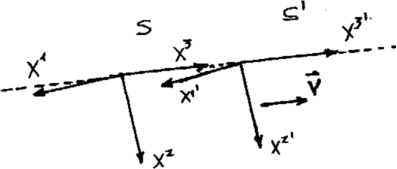
\includegraphics[width=0.4\textwidth]{images/fig_ft1_transfvec.pdf}	 
	\end{center}
	\caption{}
\end{figure} 

Se verifica entonces la transformación de Lorentz
\begin{align*}
	x^{1'} &= x^1  \\
	x^{2'} &= x^2  \\
	x^{3'} &= \gamma \: [ x^3 - \beta x^0]  \\
	x^{0'} &= \gamma \: [ x^0 - \beta x^3] 
\end{align*}
donde son 
\[
	\gamma = \frac{1}{(1 - v^2/c^2)^{1/2}} \qquad \qquad x^0 = ct 
\]

A la transformación [1] se le puede dar forma de rotación en funciones hiperbólicas como sigue
\[
	x^{0'} = x^0 \cosh( \eta ) - x^3 \sinh( \eta )
\]
\[
	x^{3'} = -x^0 \sinh( \eta ) + x^3 \cosh( \eta )
\]
donde seguimos viendo que las leyes son lineales en las coordenadas (el espacio es isótropo)
\notamargen{Debiéramos dar ideas de estas cosas importantes de relatividad especial}
\[
	\begin{pmatrix}
	 x^{0'} \\
	 x^{3'} \\
	\end{pmatrix}
	=
	\begin{pmatrix}
	\cosh( \eta ) & \sinh( \eta ) \\
	-\sinh( \eta ) & \cosh( \eta ) \\
	\end{pmatrix}
	\begin{pmatrix}
	 x^{0} \\
	 x^{3} \\
	\end{pmatrix}
\]
y no es otra cosa  que una rotación en eje $\hat{0}, \hat{3}$ con el ángulo $\eta = atanh( \beta )$. Notemos
que se verifica la invariancia del módulo de la transformación
\[
	(x^{0'})^2 -  ( (x^{1'})^2  + (x^{2'})^2 + (x^{3'})^2 ) =
		(x^{0})^2 -  ( (x^{1})^2  + (x^{2})^2 + (x^{3})^2 ) 
\]
o en una notación más feliz
\[
	(ct')^2 - ( x'^2 + y'^2 + z'^2 ) = (ct)^2 - ( x^2 + y^2 + z^2 )
\]
	
Este espacio 4D es el de Minkowski y no es euclídeo.
\[
	\begin{pmatrix}
	 x^{0'} \\
	 x^{1'} \\
	 x^{2'} \\
	 x^{3'} \\
	\end{pmatrix}
	=
	\begin{pmatrix}
	\gamma & 0 & 0 & -\beta\gamma \\
	0 & 1 & 0 & 0 \\
	0 & 0 & 1 & 0\\
	-\beta\gamma  & 0 & 0 & \gamma \\
	\end{pmatrix}
	\begin{pmatrix}
	 x^{0} \\
	 x^{1} \\
	 x^{2} \\
	 x^{3} \\
	\end{pmatrix}
\]

La transformación inversa se obtiene tomando los reemplazos
\[
	x^{i'} \to x^i \quad ,\quad  x^i \to x^{i'} \quad ,\quad  \beta \to -\beta
\]
El elemento invariante de línea es 
\[
	ds^2 = (dx^0)^2 - (dx^1)^2 - (dx^2)^2 - (dx^3)^2 = ds^{'2}
\]
o bien 
\[
	ds^2 = g_{\alpha\beta}dx^{\alpha}dx^{\beta}
\]
que es el tensor de la métrica. Se verifica
\[
	g_{\alpha\beta} = g^{\alpha\beta} =
	\begin{pmatrix}
	 1 & 0 & 0 & 0 \\
	 0 & -1 & 0 & 0 \\
	 0 & 0 & -1 & 0 \\
	 0 & 0 & 0 & -1 \\
	\end{pmatrix}
\]

\subsection{Cuadrivectores en el espacio 4D}

\subsection{Intervalos}

\begin{figure}[htb]
	\begin{center}
	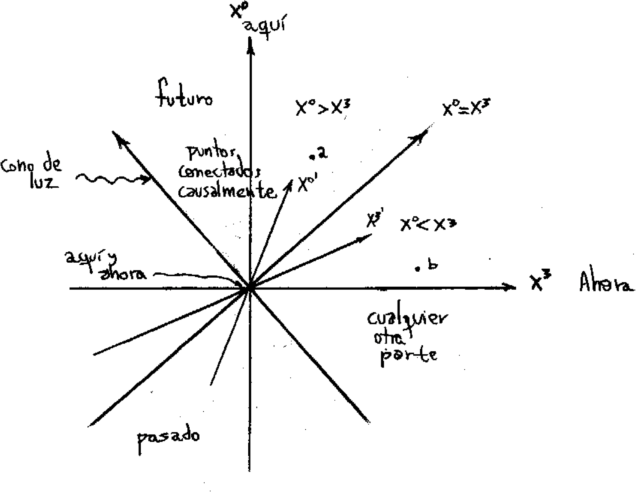
\includegraphics[width=0.4\textwidth]{images/fig_ft1_intervalos.pdf}	 
	\end{center}
	\caption{}
\end{figure} 

\subsection{Transcurso del tiempo en un sistema con V grande}

\begin{figure}[htb]
	\begin{center}
	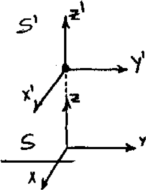
\includegraphics[width=0.4\textwidth]{images/fig_ft1_vgrande.pdf}	 
	\end{center}
	\caption{}
\end{figure} 



% =================================================================================================
\section{Transformación de los campos}
% =================================================================================================

\begin{figure}[htb]
	\begin{center}
	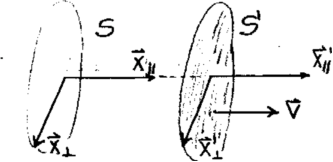
\includegraphics[width=0.4\textwidth]{images/fig_ft1_transfCampo1.pdf}	 
	\end{center}
	\caption{}
\end{figure} 

\begin{figure}[htb]
	\begin{center}
	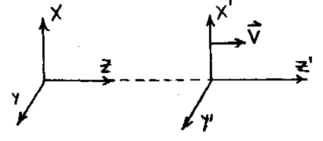
\includegraphics[width=0.4\textwidth]{images/fig_ft1_transfCampo2.pdf}	 
	\end{center}
	\caption{}
\end{figure} 



% =================================================================================================
\section{Especie de tiro oblicuo}
% =================================================================================================

\begin{figure}[htb]
	\begin{center}
	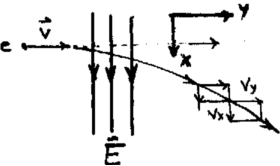
\includegraphics[width=0.4\textwidth]{images/fig_ft1_tirooblicuo.pdf}	 
	\end{center}
	\caption{}
\end{figure} 

% =================================================================================================
\section{cuadrivelocidad}
% =================================================================================================


\begin{figure}[htb]
	\begin{center}
	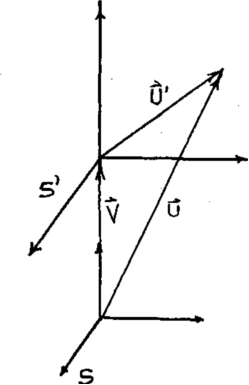
\includegraphics[width=0.4\textwidth]{images/fig_ft1_4vel.pdf}	 
	\end{center}
	\caption{}
\end{figure} 

% \bibliographystyle{CBFT-apa-good}	% (uses file "apa-good.bst")
% \bibliography{CBFT.Referencias} % La base de datos bibliográfica

\end{document}
